\documentclass[12pt]{article}
\usepackage{fontspec}
\usepackage[utf8]{inputenc}
\setmainfont{Bodoni 72 Book}
\usepackage[paperwidth=17in,paperheight=11in,margin=1in,headheight=0.0in,footskip=0.5in,includehead,includefoot,portrait]{geometry}
\usepackage[absolute]{textpos}
\usepackage{xcolor}
\usepackage{background}
\usepackage{contour}
\TPGrid[0.5in, 0.25in]{23}{24}
\parindent=0pt
\parskip=12pt
\usepackage{nopageno}
\usepackage{graphicx}
\graphicspath{ {./images/} }
\usepackage{amsmath}
\usepackage{tikz}
\newcommand*\circled[1]{\tikz[baseline=(char.base)]{
            \node[shape=circle,draw,inner sep=1pt] (char) {#1};}}

\begin{document}

\backgroundsetup{scale = 1.075, angle = 0, opacity = 0.2,
contents = {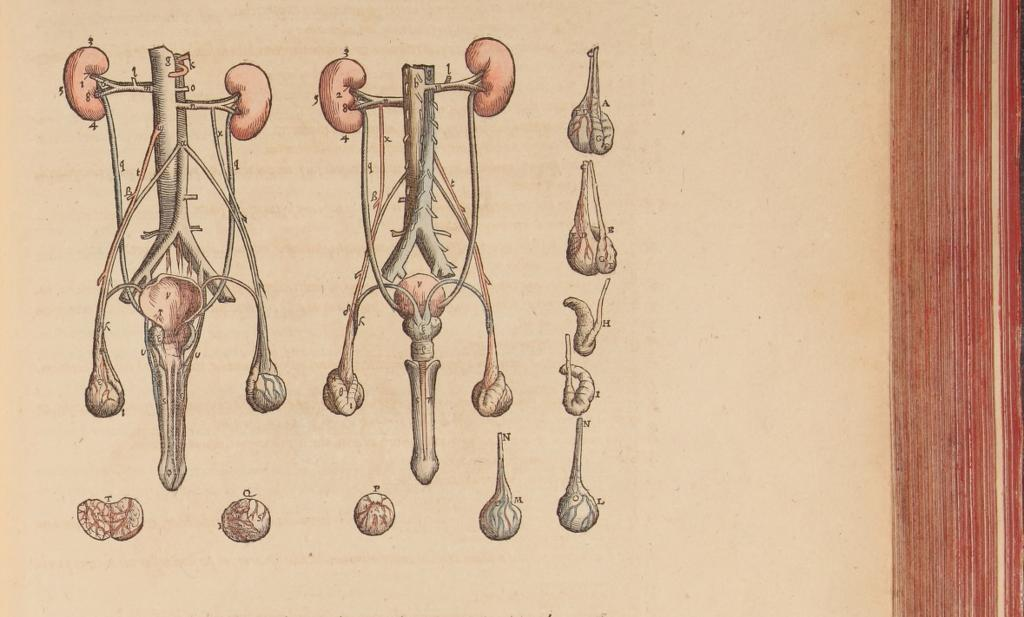
\includegraphics[width = \paperwidth,
height = \paperheight, keepaspectratio] {foreword_image.jpeg}}}

\vspace*{6\baselineskip}

\contourlength{0.04em}

\begingroup
\begin{center}
\fontsize{1.5cm}{1em} \selectfont{
\contour{white}{FOREWORD}
}
\end{center}
\endgroup

\vspace*{1\baselineskip}

\contourlength{0.07em}

\begingroup
\begin{center}
\fontsize{0.5cm}{1em} \selectfont{
\contour{white}{
\textit{``. . . v. Uesica. hæc in dextratabula priuatim adaperta est, suam commonstrans cauitatem . . .''}} \\
\contour{white}{- Andreas Vesalius}
}
\end{center}
\endgroup

\begingroup
\begin{center}
\fontsize{0.5cm}{1em} \selectfont{
\contour{white}{
{``\setmainfont{Source Han Serif SC}\selectfont. . . γ.} \textit{Meatuum urinam è renibus deducentium, in uesicam insertio.}} \\
\contour{white}{\textit{ac in dextra quidem tabula orificia, quibus hi meatus in uesicam pertinent, \& membraneiprocessus his orisicys præfecti, indicantur.}} \\
\contour{white}{\textit{in sisistra autem tabula sedes spectatur, quailli meatus primù uesica applantantur . . .''}} \\
\contour{white}{- Andreas Vesalius}
}
\end{center}
\endgroup


\end{document}